\documentclass[10pt]{article}
\usepackage[margin=0.75in]{geometry}
\usepackage{graphicx,booktabs,amsmath,hyperref,mathptmx}
\hypersetup{colorlinks=true,urlcolor=blue}
\title{Adaptive S3 rows: finite degree and relation certificates}
\author{Quadratic-twist study, PR2381}
\date{25 October 2026; adaptive-s3-20261025}
\begin{document}
\sloppy\maketitle
\noindent\textbf{Executed scope.} The preregistered adaptive row solver ran on
all 98 size-two cases, 188 main/twist base comparisons and 1,384 target
comparisons. Independent C++ and Rust agree on every polynomial witness,
matrix rank, promoted row, actual elliptic-point lift, useful coefficient
rank, stopping degree and scalar recovery. Reduced inputs have 24 target
comparisons with both higher useful rank and lower operational matrix degree;
original S3 inputs have zero. These counts are exact finite observations,
not probabilities, timings or claims of intrinsic regularity.

\section*{Actual F43 fixture}
Use $E:y^2=x^3+x$, $T:Y^2=X^3+4X$ over $\mathrm F_{43}$, order-11
generators $P=(31,18)$, $U=(24,26)$ and factor-base representatives
$(4,5),(13,19)$ and $(15,9),(17,6)$. These are existing model identities
\texttt{icv1-fp6-t0-74779950} and \texttt{icv1-fp6-t0-c6a8a47c}.
For their first targets:
\begin{center}\begin{tabular}{lrrrr}\toprule
Audited quantity & Main raw & Main reduced & Twist raw & Twist reduced\\\midrule
Useful independent rows &0&0&2&2\\
Constrained ordered roots &0&0&3&3\\
Solver matrix degree &4&3&4&2\\
Largest expanded witness degree &6&3&4&2\\
Terminal witness degree &6&3&4&2\\\bottomrule
\end{tabular}\end{center}
\noindent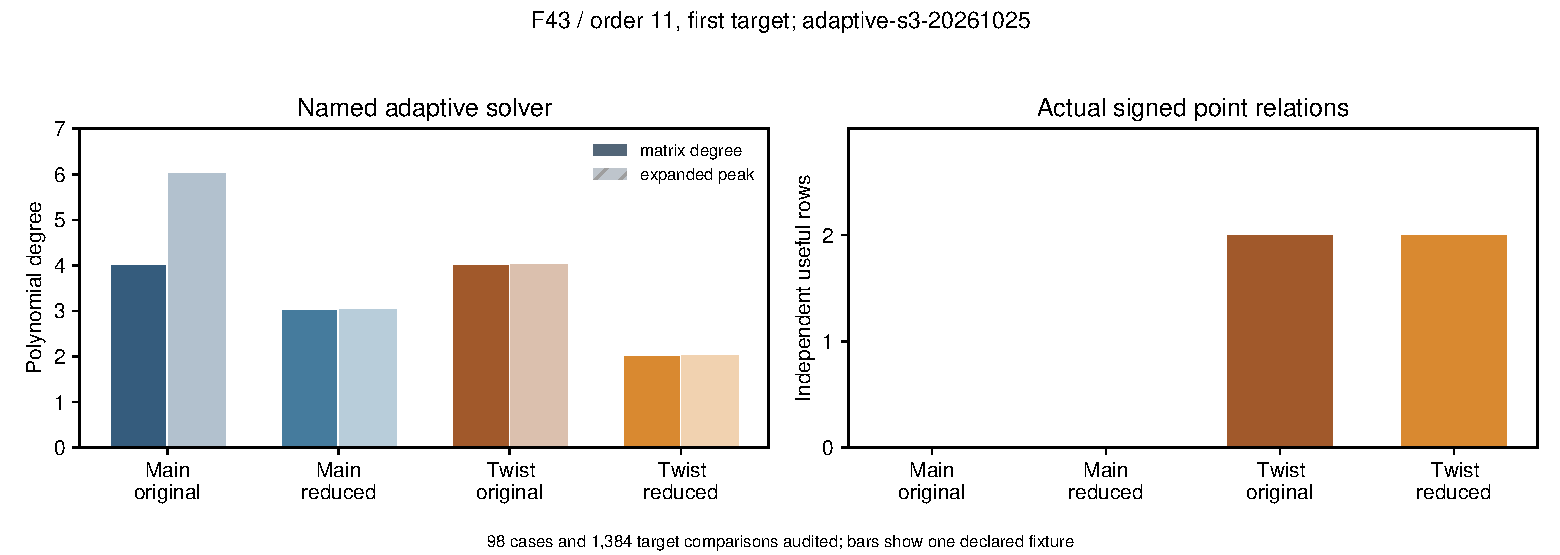
\includegraphics[width=\linewidth]{degrees.pdf}
\noindent\small Values are stored in \texttt{coverage-data.json}; the plotting
source only lays out those values. The figure shows one fixture within the
full audited population.\normalsize

\section*{What the solver certified}
The actual reduced inputs are $h_m=41xy+39(x+y)+27$,
$h_t=17xy+3(x+y)+41=17(x-15)(y-15)$, with their factor-base membership
quadratics. Each promoted row carries three exact multiplier polynomials in
the supplied inputs. The named solver builds all admissible multiples of
the pool through degree $D$, computes a full row space, reinserts a new lower
degree row only when absent from its prior lower-degree space, and rebuilds to
a fixed point. Positive acceptance requires every input active and complete
interpolation of all actual roots. Expanded witness peak includes generated
rows before reduction. Caps are explicit and none was reached.

The main reduced D=2 input space excludes 1. At D=3 the checked identity is
\[
(37+16x+16y)h_m+(21+32y)(x^2+26x+9)
 +(21+32x)(y^2+26y+9)=1\quad(\bmod\ 43).
\]
The twist has exactly the roots $(15,15),(15,17),(17,15)$; every quadratic
vanishing at them is in the span of its three input quadratics. Thus the
positive D=2 certificate and negative main D=3 certificate concern the actual
equations, rather than abstract row counts.

\section*{Source DLP and mathematical scope}
The previously proved point map $\phi(O)=O$,
$\phi(x,y)=(41x,11y)$ is an injective additive map from this main curve to
this twist, sending $P$ to $U$ and preserving integer scalars. Here it is a
base-field isomorphism. The new native routine takes each of 11 separate main
points, derives the twist base logs $5,7$ from actual generator relations,
queries the certified reduced solver on recorded target shifts, and verifies
the recovered source scalar $0,\ldots,10$ on $E$. The identity has no solver
attempt; every nonidentity attempt retains its full certificate. The solver
never receives the known-answer label.

The original-S3 main row space terminates at matrix degree 4, but its
expanded input witness reaches degree 6. This is lower \emph{operational}
matrix degree under reinsertion, not a degree-4 original-input refutation.
Both reduced arms have the same previously proved homogeneous input cutoff 2.
No intrinsic regularity separation, F4/F5 timing, asymptotic advantage or
complete ECDLP speedup is established. Different factor bases account for the
useful-rank difference in this fixture; transported-base controls identify
the relevant coordinate equivalence.

\section*{Checks and next test}
The new Lean project proves row-adjunction ideal invariance, the main D=2
dual obstruction, the D=3 unit, exact twist roots and full quadratic vanishing
space. The universal cleared unit polynomial has source-bound identity
certificate \texttt{IDC1h9eea191ebc3a8def}, checked at 32+16 native points;
false identity and source binding reject. Independent Rust checks all native
rows and recoveries. Five rehashed semantic corruptions (witness, degree,
target coverage, source and scalar) reject without an audit receipt. The
unmodified scoped proof gate and mandatory library suite were run for this
round; the exact receipts and raw failures are retained under
\texttt{validation/adaptive-s3-20261025}.

The next discriminating test uses non-isomorphic twist pairs and source-matched
bases, then charges factor-base setup, relation generation, row-space solve,
point transfer and target verification. A claim of intrinsic regularity would
need the same specified homogenization and term order on both actual ideals.
General-model normalization, exceptional S3/S4 lifting, generic pairing,
trace-zero and coordination obligations remain separate.
\end{document}
